\begin{lstlisting}
10 11 
12(3)(5)(6) 13
\end{lstlisting}
\begin{exercise}
\begin{figure}[H]
\centering

\includegraphics[width=\textwidth]{hw8-2025042123.png}
% \caption{}
\label{}
\end{figure}
\end{exercise}
\begin{proof}
由于 $f$ 是整函数,考虑它的幂级数表示形式
\[
f(z)=a_0+a_1z+a_2z^2+\dots+a_nz^{n}+\dots
\]
由 Cauchy 定理,
\[
a_n=\frac{1}{2\pi i}\oint_{C_{r}} \frac{f(z)}{z^{n+1}} \, \mathrm{d}z
\]
其中 $C_{r}$ 是以原点为中心,半径为 $r$ 的逆时针方向的圈. 对于任意 $m\geq n+1$,有
\[
\lvert a_m \rvert \leq \frac{1}{2\pi}\oint_{C_{r}} \frac{\lvert f(z) \rvert }{\lvert z \rvert ^{m+1}} \, \mathrm{d}z  \leq \frac{1}{2\pi}\oint_{C_{r}} \frac{M}{\lvert z \rvert ^{m-n+1}} \, \mathrm{d}z =\frac{M}{2\pi}\oint_{C_{r}} \frac{1}{r^{m-n+1}} \, \mathrm{d}z =\frac{M}{r^{m-n}}
\]
由 $r$ 的任意性,令 $r\to \infty$,就有 $a_m=0,\forall m\geq n+1$. 于是 $f(z)$ 是一个至多 $n$ 次的多项式或者常数.
\end{proof}

\begin{exercise}
\begin{figure}[H]
\centering

\includegraphics[width=\textwidth]{1-hw8-2025042123.png}
% \caption{}
\label{}
\end{figure}
\end{exercise}
\begin{proof}
只需要证明
\[
\lim_{ n \to \infty } \mathrm{Ln}\left( 1+\frac{z}{n} \right)^{n}=z+2k\pi i \qquad \text{for some }k\in \mathbb{Z}
\]
其中
\[
\begin{aligned}
\mathrm{Ln}\left( 1+\frac{z}{n} \right)^{n} & =n\mathrm{Ln}\left( 1+\frac{z}{n} \right) \\
 & =n\left( 2m\pi i +\sum_{k=1}^{\infty} (-1)^{k+1}\left( \frac{z}{n} \right)^{k}\frac{1}{k} \right) \\
 & =2nm\pi i+\sum_{k=1}^{\infty} (-1)^{k+1}z^{k}\cdot n^{-k+1}\cdot k^{-1} \\
\end{aligned}
\]
当 $n>2$ 时,有
\[
\begin{aligned}
\left\lvert  \sum_{k=1}^{\infty} (-1)^{k+1}z^{k}\cdot n^{-k+1}\cdot k^{-1}-z  \right\rvert  & \leq \sum_{k=2}^\infty{}\frac{\lvert z \rvert ^{k}}{n^{k-1}\cdot k} \\
 &  \leq \frac{\lvert z \rvert }{2}\sum_{k=1}^{\infty} \left( \frac{\lvert z \rvert }{n} \right)^{k}  \\
 & =\frac{\lvert z \rvert }{2}\cdot\frac{n^{-1}\lvert z \rvert }{1-n^{-1}\lvert z \rvert } \\
 & =\frac{\lvert z \rvert ^2}{2(n-\lvert z \rvert )}\to0\qquad \text{as }n\to \infty
\end{aligned}
\]
故得证!
\end{proof}

\begin{exercise}
\begin{figure}[H]
\centering
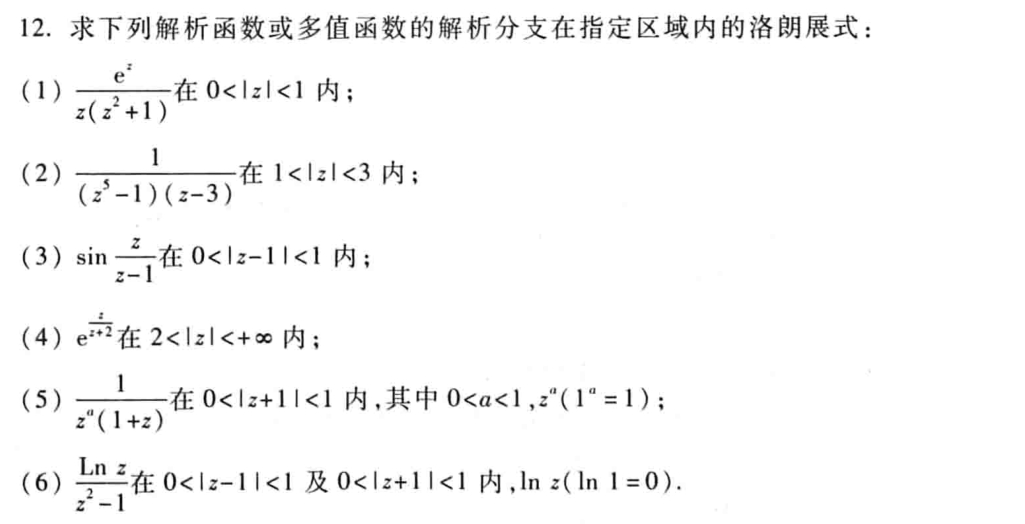
\includegraphics[width=\textwidth]{2-hw8-2025042123.png}
% \caption{}
\label{}
\end{figure}
\end{exercise}
(3)
\[
\begin{aligned}
\sin\frac{z}{z-1} & =\sin\left( 1+\frac{1}{z-1} \right) \\
 & =\sin1\cos\frac{1}{z-1}+\cos1\sin\frac{1}{z-1} \\
 & =\sum_{n=0}^{\infty} \frac{(-1)^{n}\sin1}{(2n)!\cdot(z-1)^{2n}}+\sum_{n=0}^{\infty} \frac{(-1)^{n}\cos1}{(2n+1)!\cdot(z-1)^{2n+1}}
\end{aligned}
\]
(5)
\[
\begin{aligned}
\frac{1}{z^{a}(z+1)} & =(z+1)^{-1}(-1)^{a}(1-(z+1))^{a} \\
 & =e^{ i \pi a }(z+1)^{-1} \left[ 1+\sum_{n=1}^{\infty} \frac{a(a-1)\dots(a-n+1)}{n!}(z+1)^{n} \right] \\
 & =e^{ i a \pi }(z+1)^{-1}+\sum_{n=0}^{\infty} \frac{a(a-1)\dots(a-n)}{(n+1)!}(z+1)^{n}
\end{aligned}
\]
(6) 在 $0<\lvert z-1 \rvert<1$
\[
\begin{aligned}
\frac{\mathrm{Ln}z}{z^2-1} & =\frac{\ln(1+z-1)}{(z-1)(z-1+2)} \\
 & =(z-1)^{-1} \left( \sum_{n=1}^{\infty} \frac{(z-1)^{n}(-1)^{n-1}}{n} \right)\cdot\frac{1}{2}\sum_{n=0}^{\infty} \left( -\frac{z-1}{2} \right)^{n } \\
 & =\sum_{k=0}^{\infty} \left( \sum_{n=0}^{k} \frac{(-1)^{k}}{n+1}\cdot\left( \frac{1}{2} \right)^{k-n+1} \right)\cdot(z-1)^{k} 
\end{aligned}
\]
在 $0<\lvert z+1 \rvert<1$
\[
\begin{aligned}
\frac{\mathrm{Ln}z}{z^2-1} & =\sum_{k=0}^{\infty} \left( \sum_{n=1}^{k+1} \frac{1}{n}\cdot\frac{1}{2^{k+2-n}} \right)(z+1)^{k}-i\pi\sum_{k=-1}^{\infty}\frac{(z+1)^{k}}{2^{k+2}}  \\
 & =-\frac{i\pi}{2}(z+1)^{-1}+\sum_{k=0}^{\infty}\left( \sum_{n=1}^{k+1} \frac{2^{n-k-2}}{n}-\frac{i\pi}{2^{k+2}} \right)(z+1 )^{k} 
\end{aligned}
\]
\begin{exercise}
\begin{figure}[H]
\centering
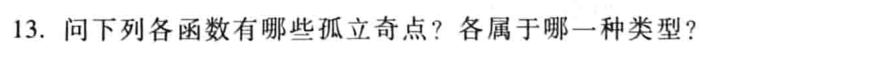
\includegraphics[width=\textwidth]{3-hw8-2025042123.png}
% \caption{}
\label{}
\end{figure}
\begin{figure}[H]
\centering
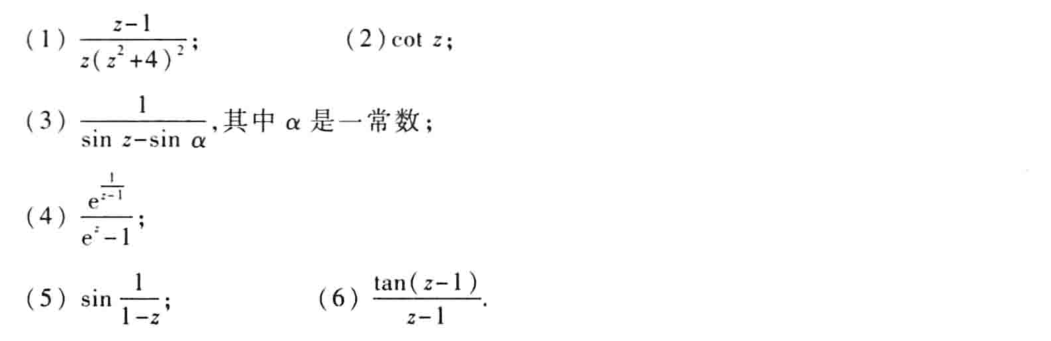
\includegraphics[width=\textwidth]{4-hw8-2025042123.png}
% \caption{}
\label{}
\end{figure}
\end{exercise}
(1)
\[
\frac{z-1}{z(z^2+4)^2}=\frac{z-1}{z(z-2i)^{2}(z-2i)^2}
\]
有孤立奇点 $0,2i,-2i,\infty$,其中 $0$ 为 1 阶极点,$2i$ 和 $-2i$ 为 2 阶极点. $\infty$ 为可去奇点.

(2)
\[
\cot z=\frac{\cos z}{\sin z}
\]
$z$ 为 $\cot z$ 奇点当且仅当 $\sin z=0$,即 $e^{ iz }=e^{ -iz }$. 也就是 $e^{ 2iz }=1$,即 $z=k\pi$ 其中 $k\in \mathbb{Z}$. 于是 $z=k\pi$,$k\in \mathbb{Z}$ 为 $\cot z$ 的孤立奇点,都是 1 阶奇点.

(3)
\[
\frac{1}{\sin z-\sin \alpha}=\frac{1}{2\sin\frac{z-\alpha}{2}\cos\frac{z+\alpha}{2}}
\]
于是孤立奇点为 $z=\alpha+2k\pi,z=\pi-\alpha+2k\pi$ 其中 $k\in \mathbb{Z}$,若 $\alpha=\pi-\alpha+2n\pi$, $n\in \mathbb{Z}$,那么 $z=\frac{\pi}{2}+2k\pi$, $k\in \mathbb{Z}$ 是所有孤立奇点,都是 2 阶极点. 否则  $z=\alpha+2k\pi,z=\pi-\alpha+2k\pi$, $k\in \mathbb{Z}$ 是所有孤立奇点,都是 1 阶极点.

(4)
\[
\frac{e^{ \frac{1}{z-1} }}{e^{ z }-1}
\]
孤立奇点为 $z=k\pi, k\in \mathbb{Z}$ 和 $z=1$,其中 $z=k\pi$ 为 1 阶极点,$z=1$ 是本性奇点.

(5)
\[
\sin\frac{1}{1-z}=\sum_{n=0}^{\infty} (-1)^{n}\frac{1}{(2n+1)!}(1-z)^{-(2n+1)}
\]
孤立奇点为 $1,\infty$,其中 $z=1$ 是本性奇点,$z=\infty$ 是可去奇点.

(6)
\[
\frac{\tan (z-1)}{z-1}=\frac{1}{\cos(z-1)}\frac{\sin(z-1)}{z-1}
\]
$\cos (z-1)=0\iff z-1=\frac{\pi}{2}+n\pi i$, 即 $z=1+\frac{\pi}{2}+n\pi i,\forall n\in \mathbb{Z}$. $z=1$ 也是奇点,但 $\lim_{ z \to 1 }\frac{\tan(z-1)}{z-1}=1$,故 $z=1$ 是可去奇点. 综上:$z=1,1+\frac{\pi}{2}+n\pi i$, $n\in \mathbb{Z}$ 是所有孤立奇点,其中 $z=1$ 是可去奇点,$z=1+\frac{\pi}{2}+n\pi i$ 是 1 阶极点
